\documentclass[../document]{subfiles}


\begin{document}
\section{Detailed Implementation Document}
\label{sec:detailed_implementation_document}

\subsection{Visualiser overview}
The visualiser takes as input from the database using what we call a controller (referring as IP controller for where the data is gathered). This data is then sorted into models and then used to make an animation. We make the animation by sending a new instruction for each frame and then use the render class to put the picture onto the stage itself. If need be, we can also change the framerate of the animation, from the standard 60 frames to anything less than 60.

\begin{figure}[H]
\centering
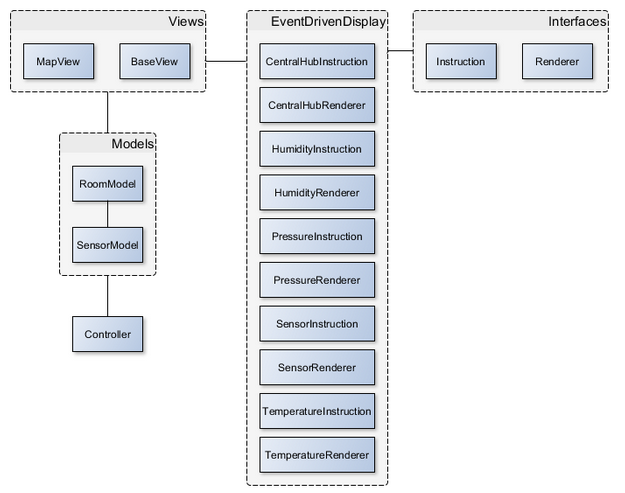
\includegraphics[width=\textwidth]{detailed_implementation/overview.png}
\caption{Overview for class diagram regarding visualiser}
\end{figure}

\subsubsection{Controller Function(CF)}

\begin{figure}[H]
\centering
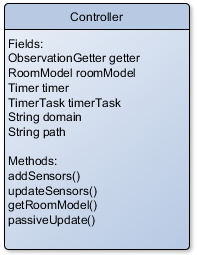
\includegraphics{detailed_implementation/controller.png}
\caption{Controller class contents}
\end{figure}

\begin{table}[H]
\caption{Controller Description}
\centering
\begin{tabularx}{\textwidth}{|l|l|X|}
	\hline
	Function nr
	&Name
	&Description
	\\ \hline CF1
	&Domain address
	&The domain address that will be used for all calls during current runtime. Most used values for our project are http://iot.altrancloud.com and localhost:4901, depending if we are using our customers database, or hosting it locally. Used to as argument under construction of getter.
	\\ \hline CF2
	&ObervationGetter
	&We are using ObservationGetter to communicate with the database for getting data. This is used every time the controller needs data from the database.
	\\ \hline CF3
	&TimerTask
	&A TimerTask is created to control how often we are pulling data from the database, the default is 5 seconds.
	\\ \hline CF4
	&RoomModel
	&RoomModel is an object where the sensorModel is stored, which is where the sensor data is stored. That is why this is the object we are updating. 
	\\ \hline CF5
	&addSensor()
	&An addSensor() method to add new sensors into the list if it is not presented earlier or at first boot up.
	\\ \hline CF6
	&updateSensors()
	&The sensor data needs to be updated each 5 seconds if the sensor object exists from before.
	\\ \hline 
\end{tabularx}
\end{table}

\subsubsection{Sensor model function (SMF)}

\begin{figure}[H]
\centering
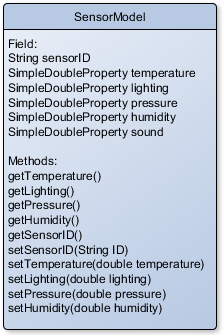
\includegraphics{detailed_implementation/sensormodel.png}
\caption{SensorModel class contents}
\end{figure}

\begin{table}[H]
\caption{SensorModel Description}
\centering
\begin{tabularx}{\textwidth}{|l|l|X|}
	\hline
	Function nr
	&Name
	&Description
	\\ \hline SMF1 
	&getTemperature()
	&Using a SimpleDoubleProperty to get the temperature.
	\\ \hline SMF2
	&getLighting()
	&Using a SimpleDoubleProperty to get the lighting
	\\ \hline SMF3
	&getPressure()
	&Using a SimpleDoubleProperty to get the pressure.
	\\ \hline SMF4
	&getHumidity()
	&Using a SimpleDoubleProperty to get the humidity.
	\\ \hline SMF5
	&getSensorID()
	&Using a String to get the sensor ID that was set by the setSensorID() method.
	\\ \hline SMF6
	&setSensorID(String ID)
	&Takes a String ID to set the sensor ID field to the correct value.
	\\ \hline SMF7
	&setTemperature(double temperature)
	&Takes a double temperature value and sets the temperature field to this value.
	\\ \hline SMF8
	&setLighting(double lighting)
	&Takes a double lighting value and sets the lighting field to this value.
	\\ \hline SMF9
	&setPressure(double pressure)
	&Takes a double pressure value and sets the pressure field to this value.
	\\ \hline SMF10
	&setHumidity(double humidity)
	&Takes a double humidity value and sets the humidity field to this value.
	\\ \hline 
\end{tabularx}
\end{table}

\subsubsection{Room Model Function (RMF)}

\begin{figure}[H]
\centering
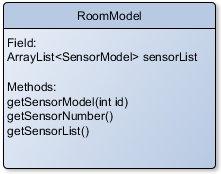
\includegraphics{detailed_implementation/roommodel.png}
\caption{RoomModel class contents}
\end{figure}

\begin{table}[H]
\caption{RoomModel Description}
\centering
\begin{tabularx}{\textwidth}{|l|l|X|}
	\hline
	Function nr
	&Name
	&Description
	\\ \hline RMF1
	&sensorModel List
	&Room model will keep an arrayList of sensorModel in order to update each sensor
	\\ \hline RMF2
	&getSensorModel(int ID)
	&A method to get a specific sensorModel using the sensorID
	\\ \hline RMF3
	&getSensorNumber()
	&getSensorNumber() will return the total number of sensor, this is useful for scaling of animation, for loops and more
	\\ \hline 
\end{tabularx}
\end{table}

\subsubsection{Base View Function (BVF)}

\begin{figure}[H]
\centering
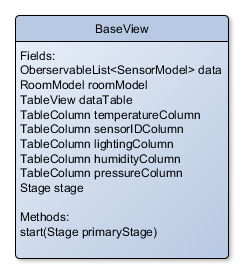
\includegraphics{detailed_implementation/baseview.png}
\caption{BaseView class contents}
\end{figure}

\begin{table}[H]
\caption{BaseView Description}
\centering
\begin{tabularx}{\textwidth}{|l|l|X|}
	\hline
	Function nr
	&Name
	&Description
	\\ \hline BVF1
	&ObservableList<SensorModel> data
	&Creates a new empty observable list that is backed by an arraylist to store data from the Sensor model.
	\\ \hline BVF2
	&start(Stage primaryStage)
	&Creates a dataTable which is a table view that is filled with data from the data list. Also adds checkboxes for the columns and listeners to make it possible to choose which columns should be visible in the dataTable.
	\\ \hline BVF3
	&main(String[] args)
	&This method starts the base view application.
	\\ \hline 
\end{tabularx}
\end{table}

\subsubsection{Map View Function (MVF)}

\begin{figure}[H]
\centering
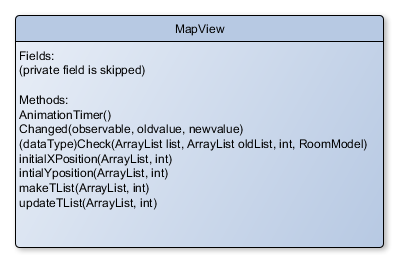
\includegraphics{detailed_implementation/mapview.png}
\caption{MapView class contents}
\end{figure}

\begin{table}[H]
\caption{Map View Description}
\centering
\begin{tabularx}{\textwidth}{|l|L{3.5cm}|X|}
	\hline
	Function nr
	&Name
	&Description
	\\ \hline MVF1
	&Image circleImage
	&Uses a String as the path for a png image used to draw the central hub.
	\\ \hline MVF2
	&start(Stage stage)
	&Draws the sensors and the central hub on the canvas and animates how the sensors changes. Also adds check boxes and listeners that is used to choose which parts of the sensor information that should be shown and descriptions of what the different parts of the drawn sensors mean.  
	\\ \hline MVF2.1
	&Canvas
	&The canvas is used to draw the animated sensors.
	\\ \hline MVF2.2
	&Central hub instruction and renderer.
	&The central hub instruction is used to set the position and image for the central hub, and the renderer is used to draw the central hub on the canvas.
	\\ \hline MVF2.3
	&AnimationTimer(now)
	&Creates a timer that is called in each frame while it is active. This timer is used to update the positions of the sensors and the values of the different sensor data.
	\\ \hline MVF2.4
	&(dataType)Instruction
	&Makes individual instructions for the data types (temperature, lighting, humidity and pressure) for every sensor to set the information related to the data type.
	\\ \hline MVF2.5
	&(dataType)Render
	&Makes individual renderers for the data types (temperature, lighting, humidity and pressure) for every sensor to be able to draw the instructions on the canvas.
	\\ \hline MVF3
	&(dataType) Check(ArrayList <Double> list, ArrayList<Double> oldList, int i, RoomModel roomModel)
	&Inserts the data belonging to the data type from the roomModel into the list on position i. Also, adds the data belonging to the data type from the roomModel into the oldList on position i if there is no data on position i yet.
	\\ \hline 
\end{tabularx}
\end{table}

\begin{table}[H]
\caption{Map View Description}
\centering
\begin{tabularx}{\textwidth}{|l|L{3.5cm}|X|}
	\hline
	MVF4
	&initialXPosition( ArrayList list, int i)
	&Adds the initial X position of sensor number i to the list.
	\\ \hline MVF5
	&initialYPosition( ArrayList list, int i)
	&Adds the initial Y position of sensor number i to the list.
	\\ \hline 
\end{tabularx}
\end{table}

\subsubsection{Instruction Function(IF)}
The instructions vary for the different instruction classes but they all have much in common. Therefore we will have all of them in one single table.
\begin{table}[H]
\caption{Instruction Function Description}
\centering
\begin{tabularx}{\textwidth}{|l|l|X|}
	\hline
	Function nr
	&Name
	&Description
	\\ \hline IF1
	&start
	&Every instruction needs a long variable start to decide when the animation needs to be played.
	\\ \hline IF2
	&length
	&Every instruction needs a long variable length that will decide how long the animation will be played.
	\\ \hline IF3
	&X and Y
	&Every instruction holds an X and Y coordinate for where the animation will be played.
	\\ \hline IF4
	&Canvas
	&Every instruction holds a canvas which is used to decide where the animation will be played.
	\\ \hline IF5
	&Check
	&Nearly all (except the centralHub) instruction comes with a boolean check, which is for the checkboxes. If the checkbox is unchecked the boolean will be false and the animation will be hidden. If the checkbox is checked the animation will continue.
	\\ \hline IF6
	&Specific function
	&Each instruction has some small differences that we will explain here.
	\\ \hline IF6.1
	&CentralHub
	&The CentralHubInstruction is presented with an image. This is because the central hub itself is static and does not need to change.
	\\ \hline IF6.2
	&Humidity
	&The HumidityInstruction needs a double for the actual humidity data. 
	\\ \hline IF6.3
	&Pressure
	&The PressureInstruction comes with the pressure data in a double format.
	\\ \hline 
\end{tabularx}
\end{table}


\begin{table}[H]
\caption{Instruction Function Description}
\centering
\begin{tabularx}{\textwidth}{|l|l|X|}
	\hline
	IF6.4
	&Sensor
	&The SensorInstruction contains the lighting data and a string that is the sensor number.
	\\ \hline IF6.5
	&Temperature
	&The TemperatureInstruction has a temperature data together with the sensor number because the user should be able to see the sensor number even if the lighting is turned off.
	\\ \hline 
\end{tabularx}
\end{table}

\subsubsection{Render Function(RF)}
\begin{table}[H]
\caption{Render Function Description}
\centering
\begin{tabularx}{\textwidth}{|l|l|X|}
	\hline
	Function nr
	&Name
	&Description
	\\ \hline RF1
	&Notify
	&The notify function will be able to take in instruction as the variable and use data from that instruction to animate the sensors on the canvas. There are many different instructions and separate renderers for each of them. Even though each renderer is different, as they all have different logic applied for animation, they all do the same thing, take an instruction and animate one single frame of the canvas.
	\\ \hline 
\end{tabularx}
\end{table}

\subsection{Database Module}
The database module support methods for opening a new connection with a database using REST, query for new data as a Observation object, and adding new data in the form of DASH7 String. The Observation class is a class taken from our customer, to better fit the format of their database.

The Altran database API is RESTful, and is accessed through simple HTTP messages. Our database implementation accesses the Altran database through this API. To send and receive HTTP messages, our implementation uses the Jersey implementation of JAX-RS (Java API for RESTful Services). The Altran database also uses Apache Lucene to implement query searches against an indexed document stored in memory, sort of like a cache. This makes it possible to pull more specific sensor data with from the database. Database queries are executed by sending HTTP GET requests with query parameters in a Lucene-specific format.

Since the visualizer needed to pull from a working database while implementing the new database, we used the old, working SQL database to do all the testing in the visualizer until we managed to integrate the new database with the visualizer.

\subsubsection{ObservationGetter(OG)}
\begin{table}[H]
\caption{Description}
\centering
\begin{tabularx}{\textwidth}{|l|L{3cm}|X|}
	\hline
	Function nr
	&Name
	&Description
	\\ \hline DBM1
	&String domain
	&The domain address that will be used for all calls during current runtime. Most used values for our project is http://iot.altrancloud.com and localhost:4901, depending if we are using our customers database, or hosting it locally. Is set during construction.
	\\ \hline DBM2
	&String path
	&The path call used to refer to the database supporting REST in the domain server. 
	\\ \hline DBM3
	&Client client
	&A javax.ws.rs.client.Client, that is the entry point which to communicate with the Jersey API.
	\\ \hline DMB4
	&WebTarget queryResource
	&The target for all requests done with Jersey, set to client.target(domain).
	\\ \hline DBM5
	&List<String> getAllSensorIDs()
	&Add “radiogateways” to the queryResource path, and split the returned DASH7 String so that only a list of radiosensorIDs remain, and return it.
	\\ \hline DBM6
	&String postD7data(String data)
	&Take a DASH7 string and post it to the server. A separate script is used for upload from sensors, so this method is used for test using mock data.
	\\ \hline DBM7
	&List<Observation> toObservationList(String jsondata)
	&Used to parse a DASH7 String response to Observation Objects.
	\\ \hline DBM8
	&Observation getMostRecentObservation(String sensorID)
	&Query the database for latest data for a sensorID using POST request with query parameter (“query”, “radiosensor:”) . Then return the observation with most recent Date value.
	\\ \hline DBM9
	&List<Observation> getRecentObservations()
	&Query the database adding “tail” to the path, to return most recent observations, uses toObservationList() to parse the result, and then return the observation with most recent Date value.
	\\ \hline DBM10
	&getQueryResult (String luceneQuery)
	&Generic method for query the database.
	\\ \hline 
\end{tabularx}
\end{table}

\subsubsection{Observation}
A model class from our customers Iot-Service project, so that our data easily follow their wanted format.

\subsection{Gateway}
In order to get the data from the sensors and push it into the database a few steps are needed to be done. First, data is retrieved from the sensors with a simple HTTP GET request to the server that runs on the Raspberry PI and the data is received in a JSON-like format. The response does not respect the protocol fully so we do not process the data, but we send it as we get it to the Altran web service which does this and inserts the data into their database. The data transmission is done through an HTTP POST request. 

All these steps are done by using shell script code and are repeated at regular intervals of time.
This approach makes sure that even if the sensors are behind a network with a firewall and a router with closed sensors, the data still reaches the database because it is our gateway that contacts the web service and not the other way around.

\end{document}